\section{Signale und Systeme}
	
	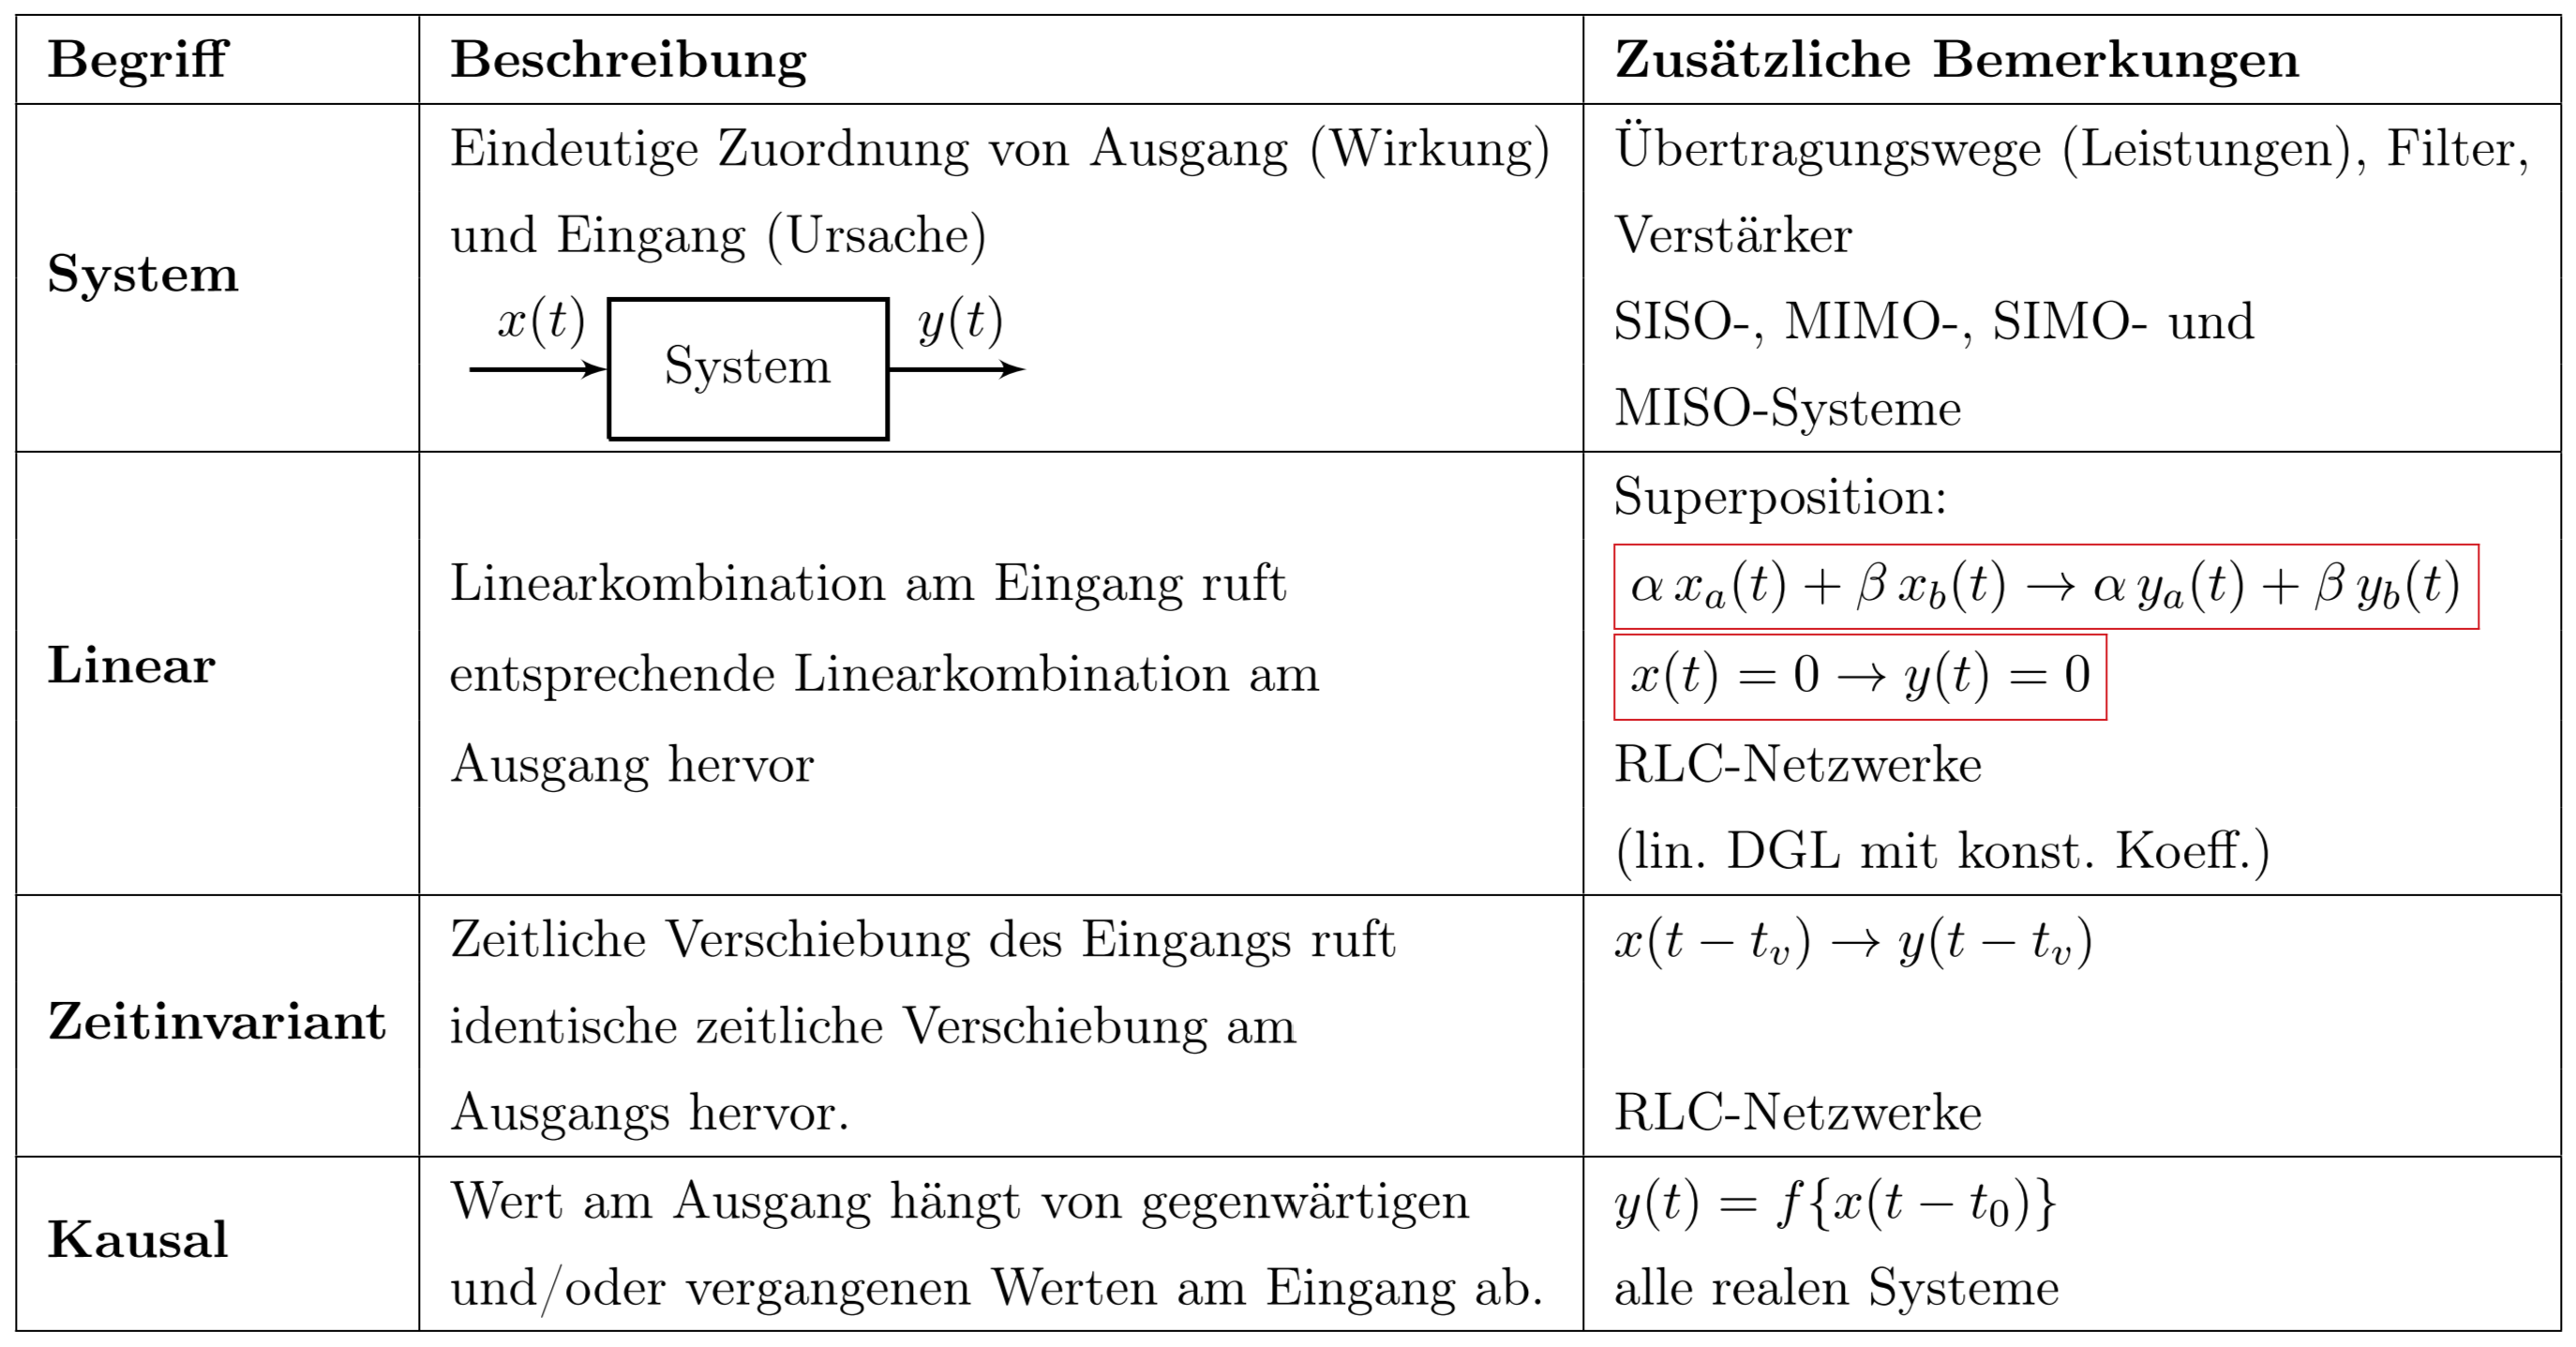
\includegraphics[width=\textwidth]{./bilder/LTISystem.png}\\

	\begin{tabular}{|l|l|}
    	\hline
    	\textbf{Linearität} & \textbf{Zeitinvarianz}\\
    	\hline
    	$\mathcal{L}(x1+x2)=\mathcal{L}(x1)+\mathcal{L}(x2)$ & $\mathcal{L}(x(t)) = y(t)$ \\
    	$\mathcal{L}(c\cdot x)=c\cdot \mathcal{L}(x)$ & $\mathcal{L}(x(t-t_0)) = y(t-t_0)$ \\
		\hline    
    \end{tabular}
  			
		
	\subsection{Lineare Systeme}
		\subsubsection{Basissignale}
			\begin{list}{$\bullet$}{\setlength{\itemsep}{0cm} \setlength{\parsep}{0cm} \setlength{\topsep}{0cm}} 
	          \item Lineare Systeme sind durch die Antworten auf die
	          Basissignale bestimmt.
	          \item Basissignale müssen linear unabhängig voneinander sein, d.h. ein
			Basissignal darf nicht durch \textbf{Linearkombination} anderer Basissignale
			darstellbar sein          
			  \item Alle möglichen Eingangs-Funktionen müssen durch eine Linearkombination der
			Basissignale dargestellt werden können. $\Rightarrow$ \textbf{Periode des Eingangssignals =	Anzahl Basissignale}
	        \end{list}
	        \vspace{.2cm}
        
		\subsubsection{Berechnung der Systemantwort aufgrund der Basissignale und der Anregung}
			\begin{enumerate}
				\item Eingangssignal $x$ als Linearkombination der Basisvektoren darstellen	$\Rightarrow$ lineares Gleichungssystem\\
				\quad $\Rightarrow x=r\cdot a + s\cdot b + t\cdot c\qquad$ ($x=$ Eingangssignal; $a,b,c=$ Basisvektoren; $r,s,t=$ Linearkombinationsparameter)\\ 
				\item Systemantwort: \quad $y=r\cdot \mathcal{L}(a) + s\cdot \mathcal{L}(b) + t\cdot \mathcal{L}(c)$ \qquad\quad $(\mathcal{L}(a)=$ Systemantwort der Basis $a$)
			\end{enumerate}
	
	\subsection{Lineare zeitinvariante Systeme (LTI-Systeme) \skript{1-5}}
	
	
%		LTI-Systeme sind durch ihre Impulsantwort $h$ vollständig bestimmt\\ \\	
%		\textbf{Berechnung der Systemantwort von diskreten LTI-Systemen}\\
%		$\; y=x*h \qquad$ ($y=$ Systemantwort; $x=$ Eingangssignal; $h=$
%		Impulsantwort)\\
%		
%		\textbf{Berechnung der Systemantwort von kontinuierlichen LTI-Systemen}\\
%		\begin{tabular}{ll}
%			\parbox{8cm}{
%			$$f_2(t) = h(t) * f_1(t) \; \laplace \; F_2(s) = H(s) \cdot F_1(s)$$
%			$$h(t) \; \laplace \; H(s)$$}
%			& \parbox{4cm}{
%		%	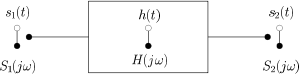
\includegraphics[width=6cm]{./bilder/utf-theorie.png}}\\
%	%	\end{tabular} \\
%	
%	\begin{tikzpicture}
%	[	inner sep = 2mm,
%	sin/.style={rectangle,minimum width=2cm,minimum height=1cm,rounded corners=5pt,draw=black,top color=white},
%	abl/.style={rectangle}
%	pil/.style={
%		->,
%		thick,
%		shorten <=2pt,
%		shorten >=2pt,}
%	]
%	
%	\node at (3,0) (L) [sin] {$\mathcal{L}$};
%	\node at (3,-1.5) (H) [sin] {$\mathcal{H}$};
%	\node at (-0.3,-0.75) {$\mathcal{F}$};
%	\node at (6.5,-0.75) {$\mathcal{F}^-1$};
%	
%	\node at (0,0) 		(ft) 	{$f(t)$};	
%	\node at (0,-1.5)	(ck)	{$ \{ c_{k} \} $};
%	\node at (6,0)		(yt) 	{$y(t)$};
%	\node at (6.5,-1.5) 	(Hw)	{$ \{ H(k \omega_0)  c_{k} \}  $};
%	
%	
%	\draw [shorten >=0.5cm,shorten <=0.5,->,thick](ft) to (L);
%	\draw [->,thick](ft) to (ck);
%
%	\draw [shorten >=0.5cm,shorten <=0.5,->,thick](ck) to (H);
%	
%	\draw [->,thick](6,-1) to (yt);
%	\draw [->,thick](4.5,0) to (5.5,0);
%	\draw [->,thick](4.5,-1.5) to (5.5,-1.5);
%	\end{tikzpicture} }
%\end{tabular} \\
%	
%
%
%    \subsection{Amplitudengang}
%        \begin{minipage}{0.3\textwidth}
%            $|H(\omega)| = \begin{cases}
%            < 1 \text{ Dämpfung} \\
%            > 1 \text{ Verstärkung}
%            \end{cases}$
%        \end{minipage}    
%        \qquad
%        \begin{minipage}{0.4\textwidth}
%            $|H(\omega)| =$ Änderung Amplitude
%        \end{minipage}
%
%	\subsection{Eigenfrequenz, Frequenzgang}
%    	Zu jeder Frequenz gehört der eigene Frequenzgang mit $a, b \in \mathbb{C}$\\
%    	$$a e^{j\omega_1 t} + b e^{j\omega_2 t} \rightarrow a H(\omega_1) e^{j\omega_1 t} + b H(\omega_2) e^{j\omega_2 t}$$
%    	Frequenzgang bei Spektraldarstellung: $$\sum_{k=-\infty}^{\infty} c_k e^{jk\omega t} \rightarrow \boxed{H(\omega)}
%    	\rightarrow \sum_{k=-\infty}^{\infty} c_k H(\omega k) e^{jk\omega t}$$			
	
	\subsection{Faltung \skript{43}}
	$y(t) = f(t)\ast g(t) = g(t) \ast f(t) = \boxed{ (f \ast g)(t) :=
	\int\limits_{-\infty}^\infty f(u) \cdot g(t-u) \, du} =
	\int\limits_{-\infty}^\infty f(t-u) \cdot g(u)\,du $ \\
	\\
	($g(t-u)$ entspricht einer Spiegelung an der Y-Achse und ist um t nach rechts geschoben)\\
	
	Hat $g\left(t\right)$ \textbf{\underline{keine} negative} Argumente dann gilt :
	$\left(g \ast f \right)\left(t\right)=\int\limits_{-\infty}^t f(u) \cdot
	g(t-u)\,du$\\
	Hat $f\left(t\right)$ \underline{keine} negative Argumente (Einschaltvorgang) dann gilt :
	$\left(g \ast f \right)\left(t\right)=\int\limits_{0}^t f(u) \cdot
	g(t-u)\,du$\\
	
	\subsubsection{Faltungssatz \skript{52}}
		\begin{minipage}{.45\textwidth}
				\begin{math}
				\boxed{
					\begin{aligned}
						\text{Zeitbereich: \quad} f(t)\cdot g(t) \; &\laplace \; \frac{1}{2\pi} \, F(\omega) \ast G(\omega) \\
						\text{Frequenzbereich: \quad} f(t) \ast g(t) \; &\laplace \; F(\omega) \cdot G(\omega) \\
					\end{aligned}
				}
				\end{math}\\
				\\
	
		\textbf{Grafische Interpretation}
		\begin{enumerate}
			\item Einfacheres Signal ($g(t)$) an der Y-Achse spiegeln
			\item Verschiebung um t nach rechts
			\item Multiplikation und Integration der beiden Signale
		\end{enumerate}
	\end{minipage}%
	\hspace{.1\textwidth}
	\begin{minipage}{.45\textwidth}
		\textbf{Bestimmung der Grenzen bei $\int\limits_{-\infty}^\infty f(u) \cdot g(t-u)\,du$}
		\begin{enumerate}
		  \item Koordinatensystem: X-Achse: t, Y-Achse: u\\ 
		  Funktion auf X-Achse: $t = t - u$, \\
		  Funktion auf Y-Achse: $t = u$
		  \item $f(u)$ unterteilen $\rightarrow$ Streifen parallel zur X-Achse
		  \item $g(t-u)$ $\rightarrow$ Streifen parallel zur $45^{\circ}$-Geraden
		  \item In u-Richtung sind die Integralgrenzen für ein \\ bestimmtes t abzulesen
		\end{enumerate}
		(siehe: Beispiel 4.2, Skript S.33)
	\end{minipage}
	
	

